\documentclass[tikz,border=20pt]{standalone}
\usepackage{xcolor}
\usetikzlibrary{positioning, arrows.meta, shapes.geometric, calc, shadows, fit, backgrounds}

% Define colors matching the AI Scientist aesthetic
\definecolor{primary}{RGB}{37, 99, 235} % blue-600
\definecolor{secondary}{RGB}{79, 70, 229} % indigo-600
\definecolor{accent}{RGB}{192, 38, 211} % fuchsia-600
\definecolor{warning}{RGB}{234, 88, 12} % orange-600
\definecolor{success}{RGB}{22, 163, 74} % green-600
\definecolor{info}{RGB}{8, 145, 178} % cyan-600
\definecolor{danger}{RGB}{225, 29, 72} % rose-600
\definecolor{bglight}{RGB}{248, 250, 252} % slate-50
\definecolor{borderlight}{RGB}{203, 213, 225} % slate-300

\begin{document}
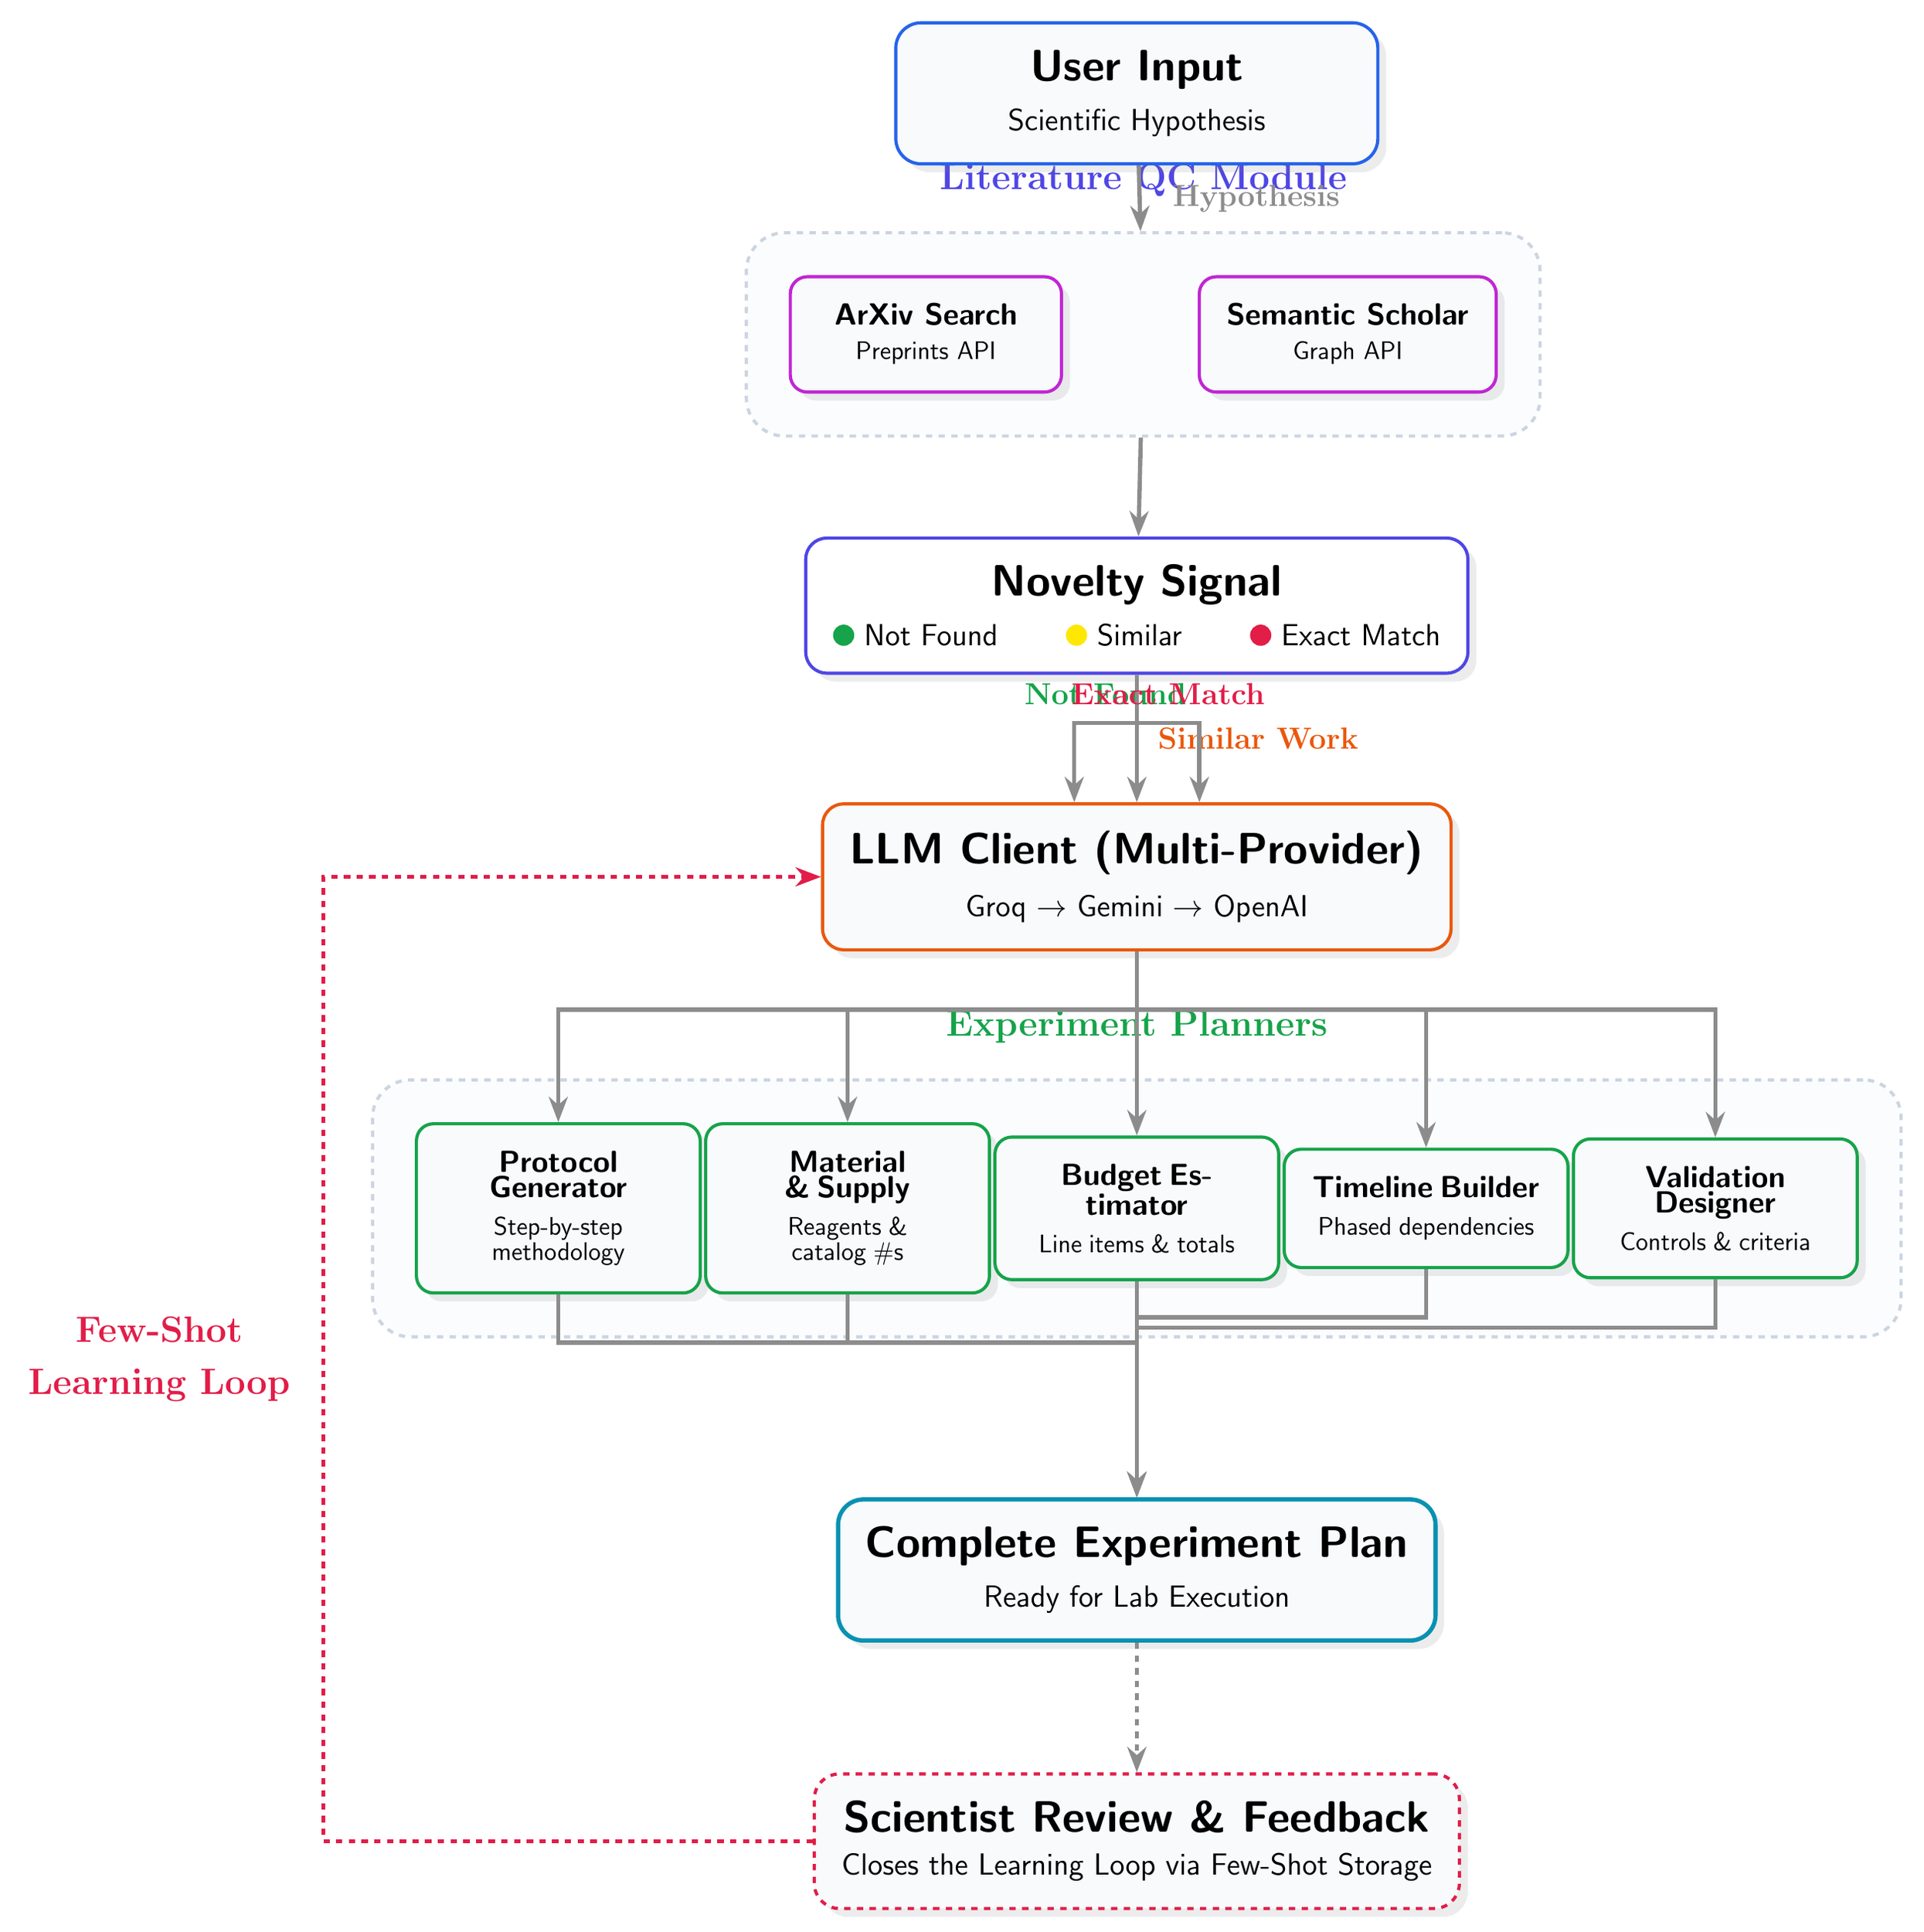
\begin{tikzpicture}[
    font=\sffamily,
    >=Stealth,
    % Styles definition
    base/.style={
        draw, thick, align=center, inner sep=3ex, 
        drop shadow={opacity=0.15, shadow xshift=4pt, shadow yshift=-4pt, color=gray}
    },
    input/.style={base, rectangle, rounded corners=12pt, fill=bglight, draw=primary, text=black, minimum width=8cm, line width=1.5pt},
    module/.style={base, rectangle, rounded corners=10pt, fill=white, draw=secondary, minimum width=9cm, line width=1.5pt},
    search/.style={base, rectangle, rounded corners=8pt, fill=bglight, draw=accent, minimum width=4.5cm, line width=1.5pt},
    llm/.style={base, rectangle, rounded corners=10pt, fill=bglight, draw=warning, minimum width=9cm, line width=1.5pt},
    generator/.style={base, rectangle, rounded corners=8pt, fill=bglight, draw=success, minimum width=4cm, text width=3.8cm, line width=1.5pt},
    final/.style={base, rectangle, rounded corners=12pt, fill=bglight, draw=info, minimum width=9cm, line width=2pt},
    feedback/.style={base, rectangle, rounded corners=12pt, fill=bglight, draw=danger, dashed, minimum width=9cm, line width=1.5pt},
    container/.style={draw=borderlight, dashed, rounded corners=18pt, fill=bglight!50, inner sep=20pt, line width=1.5pt},
    arrow/.style={->, draw=gray!80, line width=1.5pt},
    thickarrow/.style={->, draw=gray!90, line width=2pt}
]

% 1. User Input
\node[input] (user) at (0,0) {\textbf{\huge User Input}\\[3mm] \Large Scientific Hypothesis};

% 2. Literature QC Module
\node[search] (arxiv) at (-3.5, -4) {\textbf{\Large ArXiv Search}\\[1.5mm] \large Preprints API};
\node[search] (semantic) at (3.5, -4) {\textbf{\Large Semantic Scholar}\\[1.5mm] \large Graph API};

\begin{scope}[on background layer]
    \node[container, fit=(arxiv) (semantic), label={[font=\LARGE\bfseries\color{secondary}, yshift=3ex]above:Literature QC Module}] (lit_qc) {};
\end{scope}

\node[module] (novelty) at (0, -8.5) {\textbf{\huge Novelty Signal}\\[3mm] 
    \Large
    \tikz{\fill[success] (0,0) circle (5pt);} Not Found \hspace{0.8cm} 
    \tikz{\fill[yellow!90!orange] (0,0) circle (5pt);} Similar \hspace{0.8cm} 
    \tikz{\fill[danger] (0,0) circle (5pt);} Exact Match
};

% 3. LLM Orchestrator
\node[llm] (llm) at (0, -13) {\textbf{\huge LLM Client (Multi-Provider)}\\[3mm] \Large Groq $\rightarrow$ Gemini $\rightarrow$ OpenAI};

% 4. Planners
\node[generator] (protocol) at (-9.6, -18.5) {\textbf{\Large Protocol Generator}\\[2mm] \large Step-by-step methodology};
\node[generator] (materials) at (-4.8, -18.5) {\textbf{\Large Material \& Supply}\\[2mm] \large Reagents \& catalog \#s};
\node[generator] (budget) at (0, -18.5) {\textbf{\Large Budget Estimator}\\[2mm] \large Line items \& totals};
\node[generator] (timeline) at (4.8, -18.5) {\textbf{\Large Timeline Builder}\\[2mm] \large Phased dependencies};
\node[generator] (validation) at (9.6, -18.5) {\textbf{\Large Validation Designer}\\[2mm] \large Controls \& criteria};

\begin{scope}[on background layer]
    \node[container, fit=(protocol) (materials) (budget) (timeline) (validation), label={[font=\LARGE\bfseries\color{success}, yshift=3ex]above:Experiment Planners}] (planners) {};
\end{scope}

% 5. Complete Plan
\node[final] (plan) at (0, -24.5) {\textbf{\huge Complete Experiment Plan}\\[3mm] \Large Ready for Lab Execution};

% 6. Feedback
\node[feedback] (feedback) at (0, -29) {\textbf{\huge Scientist Review \& Feedback}\\[3mm] \Large Closes the Learning Loop via Few-Shot Storage};

% --- Routing / Arrows ---

% User -> Lit QC
\draw[thickarrow] (user) -- node[right=4mm, font=\Large\color{gray!90}] {\textbf{Hypothesis}} (lit_qc);

% Lit QC -> Novelty
\draw[thickarrow] (lit_qc) -- (novelty);

% Novelty -> LLM
\coordinate (n_south) at (novelty.south);
\draw[thickarrow] (n_south) -- ++(0,-0.8) coordinate (mid_n) -| node[above=1.5mm, font=\Large\bfseries\color{success}, pos=0.25] {Not Found} (llm.130);
\draw[thickarrow] (n_south) -- node[right=2mm, font=\Large\bfseries\color{warning}] {Similar Work} (llm.90);
\draw[thickarrow] (n_south) -- ++(0,-0.8) -| node[above=1.5mm, font=\Large\bfseries\color{danger}, pos=0.25] {Exact Match} (llm.50);

% LLM -> Planners
\coordinate (llm_s) at (llm.south);
\coordinate (mid_p) at (0, -15.2);
\draw[thickarrow] (llm_s) -- (mid_p) -| (protocol.north);
\draw[thickarrow] (llm_s) -- (mid_p) -| (materials.north);
\draw[thickarrow] (llm_s) -- (budget.north);
\draw[thickarrow] (llm_s) -- (mid_p) -| (timeline.north);
\draw[thickarrow] (llm_s) -- (mid_p) -| (validation.north);

% Planners -> Plan
\coordinate (plan_n) at (plan.north);
\coordinate (mid_plan) at (0, -21.8);
\draw[thickarrow] (protocol.south) -- ++(0,-0.8) -| (plan_n);
\draw[thickarrow] (materials.south) -- ++(0,-0.8) -| (plan_n);
\draw[thickarrow] (budget.south) -- (plan_n);
\draw[thickarrow] (timeline.south) -- ++(0,-0.8) -| (plan_n);
\draw[thickarrow] (validation.south) -- ++(0,-0.8) -| (plan_n);

% Plan -> Feedback
\draw[thickarrow, dashed] (plan.south) -- (feedback.north);

% Feedback -> LLM
\coordinate (fb_left) at (feedback.west);
\coordinate (llm_left) at (llm.west);
% Route safely to the left of protocol generator.
% Protocol left edge is at x = -9.6 - 2 = -11.6 approx. We route at x = -13.5.
\draw[thickarrow, dashed, draw=danger] (fb_left) -- (-13.5, -29) |- node[left=4mm, font=\LARGE\bfseries\color{danger}, pos=0.25, align=center] {Few-Shot\\[1mm]Learning Loop} (llm_left);

\end{tikzpicture}
\end{document}
